This chapter provides a theoretic view for validators, and shows how to address
internal nondeterminism by dualizing symbolic specifications.

\autoref{sec:concepts} defines the concepts in testing.  \autoref{sec:qac}
introduces a simple language that exhibits internal nondeterminism.  From
specifications written in this language, \autoref{sec:dualization} derives
validators by dualization.  The derived validators are proven correct
in \autoref{sec:proof}.

\section{Concepts}
\label{sec:concepts}
Testers are programs that determine whether implementations are compliant or not
by observing their behavior.  This section defines the basic concepts and
notations in testing.

\begin{definition}[Implementations and Behaviors]
  {\em Implementations} are programs that can interact with their environment.
  {\em Behaviors} are traces of the implementation's interactions with the
  environment and consist of (i) {\em Outputs}, which are performed by the
  implementation and can be observed in the environment, and (ii) {\em Inputs},
  which can be manipulated for testing purposes, causing (potentially) different
  outputs of the implementation.

  ``Implementation $i$ can {\em produce} behavior $b$'' is written as
  ``$\behaves i b$''.
\end{definition}

\begin{definition}[Specifications, Validity, and Compliance]
  A {\em specification} is a description of valid behavior.  ``Behavior $b$ is
  {\em valid} per specification $s$'' is written as ``$\valid s b$''.
  
  An implementation $i$ {\em complies} with a specification $s$ (written
  ``$\complies s i$'') if it only produces behaviors that are valid per the
  specification:
  \[\complies s i\quad\triangleq\quad\forall b,(\behaves i b)\implies\valid s b\]
\end{definition}

\begin{definition}[Tester components and correctness]
  A tester consists of (i) a {\em validator} that accepts or rejects
  implementations' behavior, and (ii) a {\em test harness} that triggers
  different behavior with various input.

  A tester is {\em correct} if its acceptances and rejections are sound and
  complete.  A tester is {\em rejection-sound} if it only rejects incompliant
  implementations; it is {\em rejection-complete} if it can reject all
  incompliant implementations, provided sufficient time of
  execution.\footnote{The semantics of ``soundness'' and ``completeness'' vary
    among contexts.  This paper inherits terminologies from existing
    literature~\cite{Tretmans}, but explicitly use ``rejection-'' prefix for
    clarity.  ``Rejection soundness'' is equivalent to ``acceptance
    completeness'', and vice versa.}

  The tester's correctness is based on its components properties: A
  rejection-sound tester requires its validator to be {\em rejection-sound}; A
  rejection-complete tester consists of (i) a {\em rejection-complete} validator
  and (ii) an {\em exhaustive} test harness that can eventually trigger invalid
  behavior.
\end{definition}

\begin{definition}[Soundness and completeness of validators]
  A validator $v$ is {\em rejection-sound} with respect to specification $s$
  (written as ``$\rejSound v s$'') if it only rejects behaviors that are invalid
  per $s$:
  \[\rejSound v s\quad\triangleq\quad\forall b,\rejects v b\implies\invalid s b\]

  A validator $v$ is {\em rejection-complete} with respect to specification $s$
  (written as ``$\rejComplete v s$'') if it rejects all behaviors that are
  invalid per $s$:
  \[\rejComplete v s\quad\triangleq\quad\forall b,\invalid s b\implies\rejects v b\]
\end{definition}

In property-based testing (PBT)~\cite{pbt}, validators' soundness and
completeness are trivial, because the specification itself defines ``how to
compute whether some behavior is valid or not''.  The validator is identical to
the specification.

Whereas, in model-based testing (MBT)~\cite{broy2005model}, the specification
defines ``how to produce valid behavior''.  The validator needs to compute
whether the observed behavior {\em can be produced} by the specification.

PBT and MBT are different views of the system under test: the former observes
from outside, and the latter abstracts the internal computation.  When the
system might perform nondeterministic behavior, MBT allows specifying the system
in a more reasonable way, which is explained in
\autoref{sec:challenge-nondeterminism}.

\begin{definition}[Exhaustiveness of test harness]
  A test harness $h$ is {\em exhaustive} with respect to specification $s$
  (written as ``$\exhaustive s h$'') if, for any implementation that does not
  comply with the specification, the test harness can eventually trigger some
  invalid behavior to reveal such incompliance:
  \begin{align*}
    \exhaustive s h\quad\triangleq\quad\forall i,\;&\ncomplies s i \\
    &\implies \exists b,(\triggers i h b)\wedge\invalid s b
  \end{align*}
\end{definition}

Exhaustive test harnesses can be built na\"ively by enumerating all test cases.
However, to capture bugs within realistic budget, the test harness should
produce test cases that are (i) more likely to trigger bugs, and (ii) of minimal
size to help analyzing and locating the bug.  These challenges are further
discussed in \autoref{sec:challenge-harness}.


\section{QAC language family}
\label{sec:qac}
In this section, I introduce the ``query-answer-choice'' (QAC) language family
for writing specifications and validators for network protocols that involve
internal nondeterminism.

\subsection{Specifying protocols with server models}
\label{sec:qac-model}
Network protocols can be specified with ``reference implementations'' {\it i.e.}
model programs that exhibit the space of valid behaviors.  For client-server
systems such as WWW, we can specify networked servers as programs that receive
queries and compute the responses.  Here I model the server programs with a data
structure called state monad.

\begin{definition}[State monad]
  Let $S$ be the state type, $A$ be the result type, then type $(S\to A\times
  S)$ represents a computation that, given a pre state, yields a result and the
  post state.  This computation is pronounced a ``state monad with state type
  $S$ and result type $A$''.

  For example, let the state be a key-value mapping $(K\to V)$, then we can
  define \ilc{get} and \ilc{put} computations as follows:
  \begin{align}
    \tag{1}&\mathtt{get}:K\to((K\to V)\to V\times(K\to V))\\
    \tag{2}&\mathtt{get}(k)(f)\triangleq (f(k), f)\\
    \tag{3}&\mathtt{put}:K\times V\to((K\to V)\to ()\times(K\to V))\\
    \tag{4}&\mathtt{put}(k,v)(f)\triangleq((),\update f k v)
  \end{align}

  These function definitions should be read as:
  \begin{enumerate}
    \item The \ilc{get} function takes a key as argument, and constructs a
      state monad with state type $(K\to V)$ and result type $V$.
    \item Given argument $k$ of type $K$, $\mathtt{get}(k)$ takes a mapping $f$
      as pre state and yields the mapped value $f(k)$ as result.  The post state
      is the original mapping $f$ unchanged.
    \item The \ilc{put} function takes a key-value pair as argument, and
      constructs a state monad with state type $(K\to V)$ and result type
      ``$()$'' (unit type, which corresponds to \inlinec{void} return type in
      C/Java functions).
    \item Given argument $(k,v)$ of type $(K\times V)$, $\mathtt{put}(k,v)$
      takes a mapping $f$ as pre state and substitues its value at key $k$ with
      $v$.  The post state is the substituted mapping $\update f k v$.
  \end{enumerate}
\end{definition}

Now we can define the server model in terms of state monad:

\begin{definition}[Deterministic server model]
  \label{def:qaserver}
  A deterministic server is an infinite loop whose loop body takes a query and
  produces a response.  The server definition consists of the loop body and a
  current state:
  \[\mathsf{DeterministicServer}\triangleq\sigT{S}{(Q \to S \to A \times S) \times S}\]
  This type definition is pronounced as: A deterministic server has an initial
  state of some type $S$.  Its loop body takes a request of type $Q$ and
  computes a state monad with state type $S$ and result type $A$, where type $A$
  represents the response.

  Notice that the server's state type is existentially quantified~\cite{tapl},
  while its query and response types are not.  This is because a protocol
  specification only defines the space of valid traces, and doesn't require the
  implementation's internal state to be a specific type.

  An instance of server model is written as:
  \[\existT S \sigma (\sstep,state_0)\]
  This expression is pronounced as: The server state is of type $\sigma$.  Its
  loop body is function $\sstep$ (which has type $Q\to\sigma\to A\times\sigma$)
  and its initial state is $state_0$ (which has type $\sigma$).
\end{definition}

For example, consider a compare-and-set (CMP-SET) protocol: The server stores a
number \inlinec n.  If the client sends a request that is smaller than \inlinec
S, then the server responds with \inlinec 0.  Otherwise, the server sets
\inlinec n to the request and responds with \inlinec 1:
\begin{lstlisting}[style=customc]
  int n = 0;
  while (true) {
    int request = recv();
    if (request <= n) send(0);
    else { n = request; send(1); }
  }
\end{lstlisting}

Such a server can be modelled as:
\begin{align*}
  \existT{S}{\Int}{(&\lam{(q)(n)}{\begin{cases}
        (0,s)&q\le n\\
        (1,q)&\mathrm{otherwise}
    \end{cases}},\\
    &0)}
\end{align*}

In general, servers' responses and transitions might depend on choices that are
invisible to the testers, so called internal nondeterminism, as discussed in
\autoref{sec:internal-nondeterminism}.  I represent the space of nondeterminstic
behaviors by parameterizing it over the server's internal choice.

\begin{definition}[Nondeterministic server model]
  \label{def:server}
  A nondeterministic server is an infinite loop whose loop body takes a query
  and an internal choice to produce a responses.  The nondeterministic server
  definition extends \autoref{def:qaserver} with a choice argument of type $C$:
  \[\Server\triangleq\sigT S{(Q\times C\to S\to A\times S)\times S}\]
\end{definition}

Consider changing the aforementioned CMP-SET into compare-and-reset (CMP-RST):
When the request is greater than \inlinec S, the server may reset \inlinec S to
any arbitrary number:
\begin{lstlisting}[style=customc]
  int arbitrary();
  int n = 0;
  while (true) {
    int request = recv();
    if (request <= n) send(0);
    else { n = arbitrary(); send(1); }
  }
\end{lstlisting}
Its corresponding server model can be written as:
\begin{align*}
  \existT{S}{\Int}{(&\lam{(q,c)(n)}{
      \begin{cases}
        (0,n)& q\le n\\
        (1,c)&\mathrm{otherwise}
      \end{cases}
    },\\
    &0)}
\end{align*}
This model represents the space of uncertain behavior with the internal choice
parameter of type integer.  For any value $(c:\Int)$, the server is allowed to
reset $S$ to $c$.

\subsection{Valid traces of a server model}
By specifying protocols with server models, we can now instantiate the trace
validity notation ``$\valid s t$'' in \autoref{def:compliance} in terms of
operational semantics.

\begin{definition}[Server transitions]
  \label{def:server-step}
  Upon request $q$ and choice $c$, server model $s$ can step to $s'$ yielding
  response $a$ (written ``$\triggers sc{(q,a)}s'$~'') if and only if the
  response and the post model can be computed by the $\stepServer$ function:

\begin{align*}
  &\triggers sc{(q,a)}s'\quad\triangleq\quad\stepServer(q,c)(s)=(a,s')\\
  &\stepServer:Q\times C \to \Server \to A\times \Server \\
  &\stepServer(q,c)(s)\triangleq\\
  &\qquad\letin{(\existT{S}{\sigma}{(\sstep, state)})}{s}\\
  &\qquad\letin{(a,state')}{\sstep(q,c)(state)} \\
  &\qquad(a, \existT{S}{\sigma}{(\sstep, state')})
\end{align*}

The $\stepServer$ function takes a query and a choice and computes a state monad
with state type $\Server$ and result type $A$, by pattern matching on argument
$(s:\Server)$.  Let $\sigma$ be the server state type of $s$, $\sstep$ be the
loop body, and $(state:\sigma)$ be the current state of $s$, then
$\stepServer(q,c)(s)$ computes the result $(a:A)$ and the post state
$(state':\sigma)$ using the $\sstep$ function, and substitutes the server's
pre-step $state$ with the post-step $state'$.
\end{definition}

\begin{definition}[Trace validity in QAC]
  \label{def:trace-validity}
  In the QAC language family, a trace is a sequence of $Q\times A$ pairs.  When
  specifying a protocol with a $\Server$ model, a trace $t$ is valid per
  specification $s$ if and only if it can be {\em produced} by the server model:
  \[\valid s t\quad\triangleq\quad\exists s',\behaves s t s'\]
  Here the producibility relation in \autoref{sec:concepts} is expanded with an
  argument $s'$ representing the post-transition state, pronounced
  ``specification $s$ can produce trace $t$ and step to specification $s'$~'':
  \begin{enumerate}
  \item A server model can produce an empty trace and step to itself:
    \[\behaves s \nil s\]
  \item A server model can produce a non-empty trace if it can produce the head
    of the trace, and step to some server model that produces the tail of the
    trace:
    \[\behaves s {t+(q,a)} s_2\quad\triangleq\quad\exists s_1,c,\behaves s t s_1\wedge\triggers {s_1}c{(q,a)}s_2\]
  \end{enumerate}
\end{definition}

\subsection{Validating traces}
The validator takes a trace and determines whether it is valid per the protocol
specification.

\begin{definition}[Validator]
A validator is an infinite loop whose loop body takes a pair of query and
response and determines whether it is valid or not.  The validator iterates over
a state of some type $V$.  Given a $Q\times A$ pair, the loop body may return a
next validator state or return nothing, written as type ``$\option V$'':
\[\begin{array}{lll}
  \Validator&\triangleq&\sigT{V}{(Q\times A\to V\to\option V)\times V}\\
  \option X&\triangleq&\Some(x:X)\mid\None
\end{array}\]
\end{definition}

For example, a validator for the CMP-SET protocol is written as:
\begin{align*}
  \existT{V}{\Int}{(&\lam{(q,a)(v)}{
      \begin{cases}
        \If a\Is 1\Then\Some v\Else\None&q\le v\\
        \If a\Is 1\Then\Some q\Else\None&\mathrm{otherwise}
      \end{cases}
    },\\
    &0)}
\end{align*}
Here the validator state the same as the server model's.  The loop body computes
the expected response and compares it with the observed response.  If they are
the same, then the next server state is used as the next validator state.
Otherwise, the function returns $\None$, indicating that the response is
invalid.

Having defined the validator type, we can now instantiate the trace acception
notation ``$\accepts v t$'' in \autoref{def:tester} in terms of operational
semantics.

\begin{definition}[Validator transitions]
  \label{def:validator-step}
  Validator $v$ can consume request $q$ and response $a$ and step to $v'$
  (written ``$\behaves v{(q,a)}v'$~'') if and only if the post validator can be
  computed by the $\stepValidator$ function:
\begin{align*}
  &\behaves v{(q,a)}v'\quad\triangleq\quad\stepValidator(q,a)(v)=\Some v'\\
  &\stepValidator:Q\times A\to\Validator\to\option\Validator\\
  &\stepValidator(q,a)(\existT{V}{\beta}{(\vstep,state)})\\
  &\qquad\triangleq\begin{cases}
  \Some{(\existT{V}{\beta}{(\vstep,state')})} & \vstep(q,a,state)=\Some{state'} \\
  \None & \vstep(q,a,state)=\None
  \end{cases}
\end{align*}
The $\stepValidator$ function takes a query and a response, and computes the
validator transition by pattern matching on argument $(v:\Validator)$.  Let
$\beta$ be the validator state type of $v$, $\vstep$ be the loop body, and
$(state:\beta)$ be the current state of $v$, then $\stepValidator(q,a)(v)$ calls
the $\vstep$ function to validate the $Q\times A$ pair.  If the pair is valid,
then $\vstep$ returns a post-validation $state'$, which replaces the validator's
current $state$.  Otherwise, the validator halts with $\None$.
\end{definition}

\begin{definition}[Trace acceptance in QAC]
A validator accepts a trace if it cosumes the entire trace:
\[\accepts v t\quad\triangleq\quad\exists v',\behaves v t v'\]
\begin{enumerate}
\item A validator can consume an empty trace and step to itself:
  \[\behaves v\nil v\]
\item A validator consumes a non-empty trace if it can consume the head of the
  trace, and step to some validator that consumes the tail of the trace:
  \[\behaves v {t+(q,a)} v_2\quad\triangleq\quad\exists v_1,\behaves v t v_1\wedge
  \behaves{v_1}{(q,a)}{v_2}\]
\end{enumerate}
\end{definition}


\section{Dualizing specifications into validators}
\label{sec:dualization}
As discussed in \autoref{sec:internal-external-nondeterminism}, nondeterminism
makes validators difficult to write.  To address this challenge, I construct
validators {\em automatically} from the specification.  The key idea is to
encode the specification with a programming language, and {\em dualize} the
specification program into the validator.

This chapter demonstrates the dualization technique with a programming language
in the QAC family.  \autoref{sec:encode-spec} introduces the $\Prog$ language
for encoding specifications.  Specification written in $\Prog$ are dualized into
validators in \autoref{sec:dualize-prog}, with correctness proven in
\autoref{sec:proof}.

\section{Encoding Specification Programs}
\label{sec:encode-spec}
Constructing the validator automatically requires analyzing the computations of
the specification program.  The QAC language family in \autoref{sec:qac} only
provides a state monad interface for server models, which is insufficient for
performing structural analysis.  This section introduces a programming language
for encoding specifications.

For readability, I demonstrate the dualization technique on a subset of QAC
server models called integer machine model, featuring random-access memory (RAM)
and arithmetic operations of integers.  To test real-world systems like HTTP,
I'll employ a more complex specification language in \autoref{chap:itree}.

\begin{definition}[Integer machine model]
  The server state of an integer machine model is a key-value mapping, where the
  keys are natural numbers, and the values are integers.  The initial server
  state maps all keys to zero:
  \begin{align*}
    &s_0:\Nat\to\Int\\
    &s_0=(\_\mapsto0)\\
    &\textit{i.e. }\forall (k:\Nat), s_0!k=0
  \end{align*}
  Here syntax ``$s!k$'' represents the integer value of key $(k:\Nat)$ mapped by
  $(s:\Nat\to\Int)$.

  The server's query, response, and choices ($Q$, $A$, $C$) are of type integer.
  At the beginning of each server loop, the query is written to address $!0$,
  and the internal choice is written to address $!1$.  The server then performs
  some computation that manipulates the server state, and then sends back the
  value stored in address $!0$ as the response:
\end{definition}


\[\begin{array}{lrll}
\Prog&\triangleq&\Return&\text{end computation and send response}\\
&\mid&!dst\coloneqq\Sexp;\Prog&\text{write to address }dst\in\Nat\\\null
&\mid&\If\Sexp\le\Sexp\Then\Prog\Else\Prog&\text{conditional branch}\\
\Sexp&\triangleq&\Int&\text{constant integer}\\
&\mid&!src&\text{read from address }src\in\Nat\\
&\mid&\Sexp\oop\Sexp&op\in\{+,-,\times,\div\}
\end{array}
\]

\begin{definition}[Server and validator of a program]
  A program $p\in\Lang$ is a representation of computation that can be
  ``instantiated'' into a server model:
  \[\serverOf:\Lang\to\Server\]
  
  A program can also be ``interpreted'' into other computations, including
  validators:
  \[\validatorOf:\Lang\to\Validator\]
\end{definition}

Servers specified in this $\Prog$ language are defined as follows:
\begin{enumerate}
\item The server's query, response, and choices ($Q$, $A$, $C$) are all
  natural numbers.
  \[\serverOf(p)\triangleq\existT{S}{\Nat\to\Int}{(\sstep_p,(\_\mapsto0))}\]
\item At the beginning of each server loop, the query is written to address
  $!0$, and the internal choice is written to address $!1$.
\item After writing the query and response, the server $\Exec$utes the $\Prog$
  model, which manipulates the key-value store.
\item When the $\Prog$ model $\Return$s, the server sends back the value stored
  in address $!0$ as the response.
\end{enumerate}
Let $p\in\Prog$ be the model program, then the server's loop body $\sstep_p$ is
defined as:
\[\begin{array}{lr@{\,}l}
\sstep_p(q,c,s_0)&\triangleq&\letin{s_1}{\update{s_0}{1}{c}}\\
&&\letin{s_2}{\update{s_1}{0}{q}}\\
&&\letin{s_3}{\Exec(p,s_2)}\\
&&(s_3!0,s_3)\\
\Exec(p,s)&\triangleq&
\begin{cases}
  s&p\Is\Return\\
  \Exec(p',\update{s}{dst}{e^s})&p\Is !dst\coloneqq e;p'\\
  \Exec(\If {e_1}^s\le{e_2}^s\Then p_1\Else p_2,s)&p\Is\If e_1\le e_2\Then p_1\Else p_2
\end{cases}\\
e^s&\triangleq&
\begin{cases}
  z&e\Is z:\Int\\
  s!src&e\Is !src\\
  {e_1}^s\oop{e_2}^s&e\Is e_1\oop e_2
\end{cases}
\end{array}\]
Here ``$e^s$'' is pronounced ``evaluating server expression $(e:\Sexp)$ with
state $(s:\Nat\to\Int)$''.  It substitutes all occurences of ``$!src$'' with the
value stored at address $src$ of mapping $s$, written as ``$s!src$''.
``$s[k\mapsto v]$'' is pronounced ``updating mapping $s$ at address $k$ to value
$v$''.  It produces a new state where $k$ is mapped to $v$, while other
addresses remain unchanged from $s$:
\[s[k\mapsto v]!k'\triangleq\begin{cases}v&k'=k\\
s!k'&k'\neq k\end{cases}\]

To specify protocols with this $\Prog$ language, the model program should read
the query from address $!0$, and parameterize the space of nondeterministic
behavior over the internal choice in address $!1$.  When the model program
returns, it should have stored the computed response in address $!0$.  Addresses
greater than $!1$ are only writable by the specification, and can be used for
storing the server state.

For example, the CMP-RST specification in \autoref{sec:qac} can be written in
$\Prog$ as:
\[\begin{array}{ll}
\If !0\le!2\Then !0\coloneqq0;\Return&(1)\\
\eelse!0\coloneqq1;!2\coloneqq!1;\Return&(2)
\end{array}\]
When the query is less than or equal to the value stored in $!2$ (case 1), the
server writes response $0$ to address $!0$, and leave address $!2$ untouched.
For queries greater than the value in $!2$ (case 2), the server writes $1$ as
response, and updates address $!2$ with the internal choice stored in $!1$.

This $\Prog$ language features arithmetic operations, conditional branches,
memory access, and internal nondeterminism.  It also exhibits a tree structure
that allows inductive reasoning.  The rest of this section derives validators
from $\Prog$ models, and prove the correctness of such derived validators.

\section{Dualize model program into validator}
\label{sec:dualize-prog}
The validator of a model $p\in\Prog$ needs to determine whether the trace is
producible by $p$.  More specifically, whether the responses in the trace can be
{\em explained} by $p$'s return value stored at address $!0$.

The idea is similar to \ilc{tester} in \autoref{sec:interactive-testing}, which
\ilc{validate}s the trace by executing the \ilc{serverSpec}, and comparing the
expected response against the tester's observation.

However, when the specification is nondeterministic, the expectation of response
$A$ is parameterized over the internal choice $C$.  Therefore, the validator
should determine whether there exists such $C$ that led the specification to
produce the observed $A$.

This reduces the trace validation problem to constraint solving.  Upon observing
a response, the validator adds a constraint that the observation can be
explained by running the specification with certain value of choices.

More specifically, the validator executes the $\Prog$ model and represents
internal choices with {\em symbolic variables}.  These variables are carried
along the program execution, so the expected responses are computed as {\em
  symbolic expressions} that might depend on those variables.  The validator
then constraints that the symbolic response is equal to the concrete
observation.

To achieve this goal, the validator needs to store the symbolic expression for
each address of the server model.  It also needs to remember all the constraints
added upon observation.  I store these information as ``validation states'':
\[(\Nat\to\Vexp)\times\Set\constraint\]
Here the $\constraint$s are relations between validator expressions ($\Vexp$s)
that may depend on symbolic $\Var$iables:
\[\begin{array}{lrl@{\qquad}l}
\constraint&\triangleq&\Vexp\ccmp\Vexp&cmp\in\{<,\le,\equiv\}\\
\Vexp&\triangleq&\Int&\text{constant integer}\\
&\mid&\#x&\text{variable }x\in\Var\\
&\mid&\Vexp\oop\Vexp&op\in\{+,-,\times,\div\}\\
\end{array}\]

In practice, I use an equivalent definition for the validator state:
\[(\Nat\to\Var)\times\Set\constraint\]
The key-expression mapping $(k\mapsto e)$ above can be simulated with the
key-variable $(k\mapsto x)$ mapping here, by adding $(\#x\equiv e)$ to the set
of constraints.  I alter the type interface for convenience of developing the
validator.

Notice that the internal choices might affect branch conditions, so the
validator doesn't know which branch in the specification was taken.  Therefore,
it should maintain multiple validation states, one for each possible execution
path of the specification:
\[\Set((\Nat\to\Var)\times\Set\constraint)\]

The initial state of the validator is a single validation state that corresponds
to the specification's initial state:
\[\{(\_\mapsto\#0,\{\#0\equiv0\})\}\]
Here the initial validation state says ``all addresses are mapped to variable
$\#0$, and the value of variable $\#0$ is constrained to be zero''.  This
reflects the initial server state that maps all addresses to zero value.

The validator's loop body is derived by dualzing the server model:

\begin{figure}[h]
\[\begin{array}{l@{\;}r@{\;}l}
\validatorOf(p)&\triangleq&\existT{V}{\Set((\Nat\to\Var)\times\Set\constraint)}{\\
  &&(\vstep_p,\{(\_\mapsto\#0,\{\#0\equiv0\})\})}\\
\vstep_p(q,a,v)&\triangleq&\letin{v'}{v_0\gets v;\vstep'_p(q,a,v_0)}\\
&&\If v'\Is\varnothing\Then\None\Else\Some v'\hfill(\ref{rule:reject})\\
\vstep'_p(q,a,v_0)&\triangleq&\letin{v_1}{\Havoc(1,v_0)}\\
&&\letin{v_2}{\Write(0,q,v_1)}\\
&&(vs_3,cs_3)\gets\Exec(p,v_2);\\
&&\letin{cs_4}{cs_3\cup\{\#(vs_3!0)\equiv a\}}\hfill(\ref{rule:return})\\
&&\If\solvable cs_4\Then\{(vs_3,cs_4)\}\Else\varnothing\hfill(\ref{rule:unsat})\\
\Exec(p,(vs,cs))&\triangleq&\begin{cases}
  \{(vs,cs)\}&p\Is\Return\\
  \Exec(p',\Write(d,e,(vs,cs)))&p\Is !d\coloneqq e;p'\\
  \left(\begin{array}{@{}l}
    \letin{v_1}{(vs,cs\cup\{{e_1}^{vs}\le{e_2}^{vs}\})}\\
    \letin{v_2}{(vs,cs\cup\{{e_2}^{vs}<{e_1}^{vs}\})}\\
    \Exec(p_1,v_1)\cup\Exec(p_2,v_2)\hfill(\ref{rule:branch})
  \end{array}\right)&\begin{array}{@{}l}p\Is\\
    \If e_1\le e_2\\
    \tthen p_1\Else p_2\end{array}
\end{cases}\\
\Write(d,e,(vs,cs))&\triangleq&\letin{x_e}{\Fresh (vs,cs)}\hfill(\ref{rule:write})\\
&&(\update{vs}{d}{x_e},cs\cup\{\#x_e\equiv e^{vs}\})\\
\Havoc(d,(vs,cs))&\triangleq&\letin{x_c}{\Fresh (vs,cs)}(\update{vs}{d}{x_c},cs)\hfill(\ref{rule:choice})\\
e^{vs}&\triangleq&\begin{cases}
  n&e\Is n:\Nat\\
  \#(vs!src)&e\Is!src\\
  {e_1}^{vs}\oop{e_2}^{vs}&e\Is e_1\oop e_2
\end{cases}
\end{array}\]
\caption[Dualizing server model into validator]{Dualizing server model into
  validator, with derivation rules annotated.}
\label{fig:dualize}
\end{figure}

\begin{enumerate}
\item \label{rule:write} When the server performs a write operation
  $!dst\coloneqq exp$, the validator creates a fresh variable $x$ to represent
  the new value stored in address $!dst$, and adds a constraint that says $x$'s
  value is equal to that of $exp$.
\item \label{rule:branch} When the server makes a nondeterministic branch $\If
  e_1\le e_2\Then p_1\Else p_2$, consider both cases: (a) If $p_1$ was taken,
  then the validator should add a constraint $e_1\le e_2$; or (b) If $p_2$ was
  taken, then the validator should add constraint $e_2<e_1$.
\item \label{rule:choice} Before executing the program, the server writes the internal
    choice $c$ to address $!1$.  Accordingly, the validator creates a fresh
    variable to represent the new value stored in address $!1$, without adding
    any constraint.
\item \label{rule:return} After executing the program, the server sends back the
  value stored in $!0$ as response.  Accordingly, the validator adds a
  constraint that says the variable representing address $!0$ is equal to the
  observed response.
\item \label{rule:unsat} When the constraints of a validation state becomes
  unsatisfiable, it indicates that the server model cannot explain the
  observation.  This is because either (i) the observation is invalid {\it i.e.}
  not producible by the server model, or (ii) the observation is valid, but was
  produced by a different execution path of the server model.
\item \label{rule:reject} The validator accepts the trace if it can be produced
  by any execution path of the server model.  Since each execution path
  corresponds to a validation state, the validator only needs to remove the
  unsatisfiable state from the set of states.  If the set of validation states
  becomes empty, it indicates that the observation cannot be explained by any
  execution path of the specification, so the validator should reject the trace.
\end{enumerate}

This mechanism is formalized in \autoref{fig:dualize}.  Here notation
``$v_0\gets v;\vstep'_p(q,a,v_0)$'' is a monadic bind for sets: Let $\vstep'_p$
map each element $v_0$ in $v$ to a set of validation states
$(\vstep'_p(q,a,v_0):\Set((\Nat\to\Var)\times\Set\constraint))$, and return the
union of all result sets as $v'$.

The validator assumes a constraint solver that can determine whether a set of
constraints is satisfiable, {\it i.e.} whether there exists an {\em assignment}
of variables $(\Var\to\Int)$ that satisfy all the constraints:
\begin{gather*}
  \forall cs,\solvable cs\iff\exists (asgn:\Var\to\Int),\satisfy{asgn}cs\\
  \begin{array}{r@{\;}l}
    \satisfy{asgn}cs\triangleq&\forall(e_1\ccmp e_2)\in cs, {e_1}^{asgn}\ccmp{e_2}^{asgn}\\
    e^{asgn}\triangleq&\begin{cases}
      z&e\Is z:\Int\\
      asgn!x&e\Is \#x\\
      {e_1}^{asgn}\oop{e_2}^{asgn}&e\Is e_1\oop e_2
    \end{cases}
  \end{array}
\end{gather*}
Here ``$e^{asgn}$'' is pronounced ``evaluating validator expression $(e:\Vexp)$
with assignment $(asgn:\Var\to\Int)$''.  It substitutes all occurences of
``$\#x$'' with their assigned value $(asgn!x)$.

When the $\Prog$ model writes to memories or makes conditional branches, the
operands are represented as specification expressions ($\Sexp$) that refer to
server addresses.  To construct the constraints over symbolic variables, the
validator translates the expressions $(e:\Sexp)$ into validator expressions
$(e^{vs}:\Vexp)$ by {\em symbolizing} it with the validation state
$(vs:\Nat\to\Var)$, which substitutes all addresses $(!src)$ with their
corresponding variable $\#(vs!src)$.

\begin{figure}[h]
\begin{align*}
&\validatorOf(\texttt{CMP-RST})\triangleq\existT{V}{\Set((\Nat\to\Var)\times\Set\constraint)}\\
  &\begin{array}{rll}
     (&\lam{(q,a,v)}{&\llet v'=\begin{array}[t]{@{}l@{}l@{}ll}
       \multicolumn{3}{@{}l}{(vs_0,cs_0)\gets v;}\\
       \letin{vs_1&}{\update{vs_0}{1}{\Fresh (vs_0,cs_0)}&}&\text{(1)}\\
       \letin{x_q&}{\Fresh (vs_1,cs_0)&}\\
       \letin{vs_2&}{\update{vs_1}{0}{x_q}&}\\
       \letin{cs_2&}{cs_0\cup\{\#x_q\equiv q\}&}\\
       \letin{cs_{3a0}&}{cs_2\cup\{\#(vs_2!0)\le\#(vs_2!2))\}&}&\text{(2a)}\\
       \letin{x_{3a1}&}{\Fresh (vs_2,cs_{3a0})&}\\
       \letin{vs_{3a1}&}{\update{vs_2}{0}{x_{3a1}}&}\\
       \letin{cs_{3a1}&}{cs_{3a0}\cup\{\#x_{3a1}\equiv0\}&}\\
       \letin{cs_{3b0}&}{cs_2\cup\{\#(vs_2!2)<\#(vs_2!0)\}&}&\text{(2b)}\\
       \letin{x_{3b1}&}{\Fresh (vs_2,cs_{3b0})&}\\
       \letin{vs_{3b1}&}{\update{vs_2}{0}{x_{3b1}}&}\\
       \letin{cs_{3b1}&}{cs_{3b0}\cup\{\#x_{3b1}\equiv1\}&}\\
       \letin{x_{3b2}&}{\Fresh (vs_{3b1},cs_{3b1})&}\\
       \letin{vs_{3b2}&}{\update{vs_{3b1}}{2}{x_{3b2}}&}\\
       \letin{cs_{3b2}&}{cs_{3b1}\cup\{\#x_{3b2}\equiv\#(vs_{3b2}!1)\}&}\\
       \multicolumn{3}{@{}l}{((vs_4,cs_4)\gets\{(vs_{3a1},cs_{3a1}),(vs_{3b2},cs_{3b2})\};}&\text{(3)}\\
       \letin{cs_5&}{cs_4\cup\{\#(vs_4!0)\equiv a\}&}\\
       \multicolumn{3}{@{}l}{\If\solvable cs_5\Then\{(vs_4,cs_5)\}\Else\varnothing}\\
       \end{array}\\
       &&\iin\\
       &&\If v'\Is\varnothing\Then\None\Else\Some v'
     }\\
     ,&\multicolumn{2}{l}{\{(\_\mapsto\#0,\{\#0\equiv0\})\}})
   \end{array}
\end{align*}
\caption[Validator for protocol CMP-RST]{Validator for CMP-RST, derived from
  $\Prog$ model.  This program consists of three parts: (1) symbolizing the
  query and internal choice before executing the model, (2) considering both
  branches in the model program, propagating a validation state for each branch,
  (3) filtering the validation states by constraint satisfiability, removing
  invalid states.}
\label{fig:derived-validator}
\end{figure}

For example, by dualizing the $\Prog$ model for CMP-RST in
\autoref{sec:proglang}, we get a validator as shown in
\autoref{fig:derived-validator}.  Such derived validators are proven sound and
complete in the following section.

\section{Correctness Proof}
\label{sec:proof}
Validators derived in this approach can be proven sound and complete:
\[\begin{array}{r@{\;}l}
\forall p:\Prog,&\letin{s}{\serverOf(p)}\\
&\letin{v}{\validatorOf(p)}\\
&\rejSound v s\wedge\rejComplete v s\\
&\text{\it i.e. }\forall t:\List(Q\times A),\\
&\qquad\valid s t\iff\accepts v t\\
&\qquad\text{\it i.e. }\exists s',\behaves s t s'\iff\exists v',\behaves v t v'
\end{array}\]

In this subsection, I first present a generic framework for proving validators'
correctness properties, and then demonstrate its usage by applying it to
$\Prog$-based validators.

The ``equivalence between server production and validator consumption of all
traces'' is proven by introducing a loop invariant.  The invariant is a
bisimulation between the server and the validator, which is preserved for each
step of the trace produced/consumed.

\subsection{Proving rejection soundness}
The proof of ``any trace produceable by the server is consumable by the
validator'' is by forward induction on the server's execution path.  The
corresponding validation path is constructed based on the following hypotheses:
\begin{itemize}
\item The initial server state reflects the initial validator state:
  \begin{equation}
    \tag{RejSound1}
    \label{eq:rs1}
    \Reflects{(v_0:V)}{(s_0:S)}
  \end{equation}
\item Any server step whose pre-execution state reflects some pre-validation
  state can be consumed by the validator into a post-validation state that
  reflects the post-execution state:
  \begin{align*}
    \tag{RejSound2}
    \label{eq:rs2}
    &\forall(q:Q)(c:C)(a:A)(s,s':S)(v:V),\\
    &\sstep(q,c,s)=(a,s')\wedge\Reflects{v}{s}\\
    &\implies\exists v':V,\vstep(q,a,v)=\Some{v'}\wedge\Reflects{v'}{s'}
  \end{align*}
  \begin{center}
    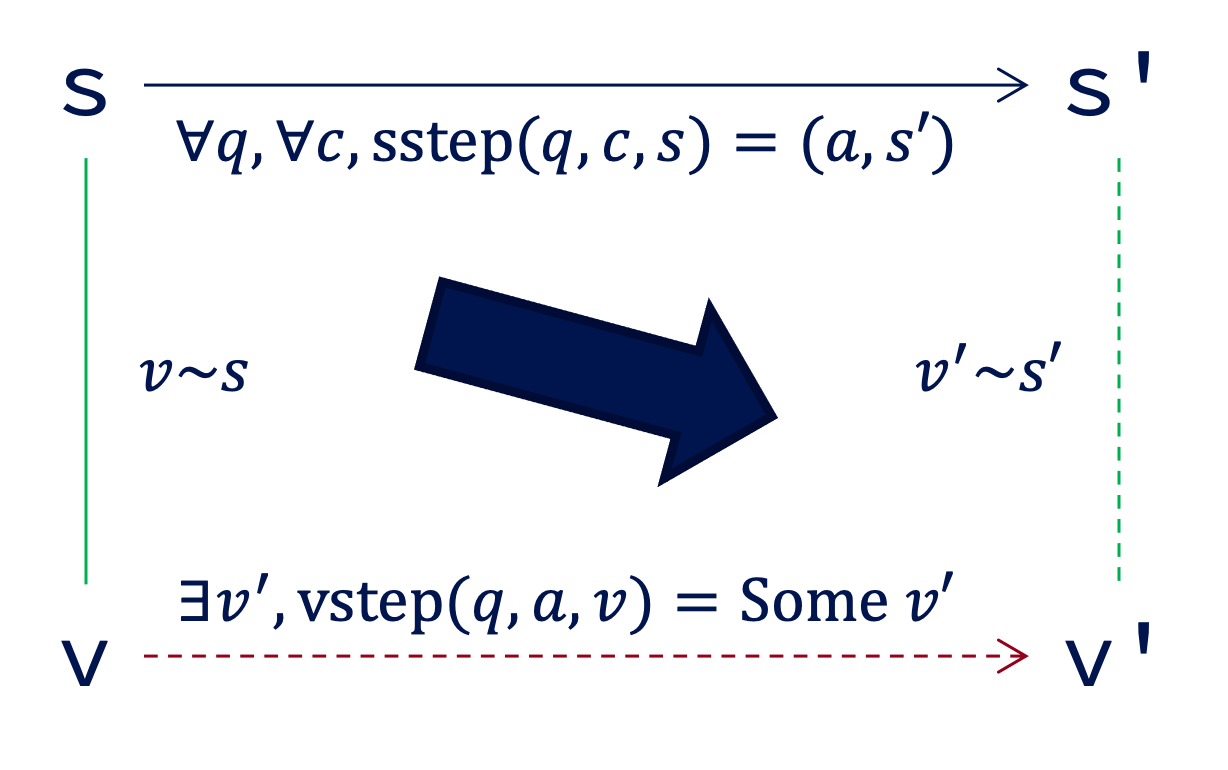
\includegraphics[width=.5\textwidth]{figures/sound}
  \end{center}
\end{itemize}

\subsection{Proving rejection completeness}
The proof of ``any trace consumable by the validator is produceable by
the server'' is by backward induction on the validator's execution
path.  The corresponding server path is constructed based on the
following hypotheses:

\begin{itemize}
\item Any accepting validator step has some server state that reflects the
  post-validation state:
  \begin{align*}
    \tag{RejComplete1}
    \label{eq:rc1}
    \forall(q:Q)(a:A)(v, v':V),\;&\vstep(q,a,v)=\Some{v'}\\
    &\implies\exists s':S,\Reflects{v'}{s'} 
  \end{align*}
\item Any accepting validator step whose post-validation state reflects some
  post-execution server state has a corresponding server step from a
  pre-execution state that reflects the pre-validation state:
  \begin{align*}
    \tag{RejComplete2}
    \label{eq:rc2}
    &\forall(q:Q)(a:A)(v,v':V)(s':S),\\
    &\vstep(q,a,v)=\Some{v'}\wedge\Reflects{v'}{s'}\\
    &\implies\exists(s:S)(c:C),\sstep(q,c,s)=(a,s')\wedge\Reflects{v}{s}
  \end{align*}
  \begin{center}
    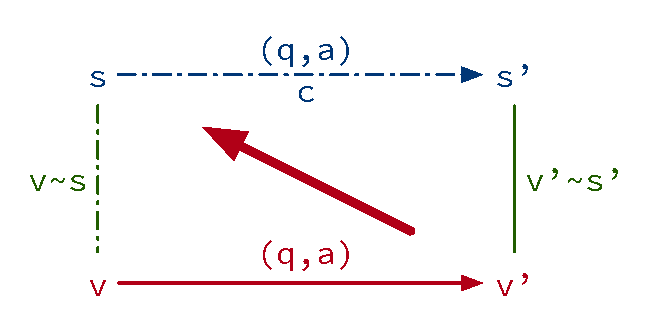
\includegraphics[width=.5\textwidth]{figures/complete}
  \end{center}

\item The initial validator state only reflects the initial server state:
  \begin{equation}
    \tag{RejComplete3}
    \label{eq:rc3}
    \{s\mid\Reflects{v_0}{s}\}=\{s_0\}
  \end{equation}
\end{itemize}

Rejection soundness is proven by forward induction, while rejection completeness
is proven by backward induction.  This is because the choice $c$ is known from
the server step, while unknown from the validator step: Given a validator step,
we cannot predict ``what choices the server will make in the future'', but can
analyze ``what choices the server might have made in the past''.  This proof
method is further explained with the $\Prog$ example:

For specifications written in the $\Prog$ language, the server state is a
mapping from addresses to data; the validation state is a mapping from addresses
to symbolic variables, and constraints over the variables.  A validation state
is accepting if its constraints are satisfiable, {\it i.e.}  there exists an
{\em assignment} of the symbolic variables that can unify the trace with the
server model.  The internal choices made by the server are represented as
symbolic variables.  The assignment maps these variables to the choices' value
at each step, from which we can reconstruct the server's execution path.
\begin{definition}[Bisimulation for $\Prog$ specifications]
  Validator state $v$ {\em simulates} server state $s$ if it contains a
  validation state $(vs,cs)$ that {\em reflects} the server state: (1) There
  exists an assignment $asgn$ that can satisfy the constraints $cs$; and (2) The
  address-variable mapping $vs$ can be {\em instantiated} with the assignment
  (written as ``$vs^{asgn}$'') into an address-data mapping that is equivalent
  with $s$:
  \begin{align*}
    \Reflects v s\quad\triangleq\quad& \exists((vs,cs)\in v)(asgn:\Nat\to\Nat),\satisfy{asgn}
    cs\wedge vs^{asgn}=s\\ vs^{asgn}\quad\triangleq\quad&addr\mapsto
    asgn!(vs!addr)
  \end{align*}
\end{definition}
This bisimulation definition satisfies the hypotheses for proving soundness and
completeness:

Hypotheses~\ref{eq:rs1} and \ref{eq:rc3} are immediate from the initial states'
definition: The initial server state is all-zero map.  The initial validator
state is a singleton that maps all addresses to a variable that is constrained
to have value zero.

\autoref{eq:rc1} is based on the fact that $\vstep_p$ checks the nonemptiness of
the result:
\[\forall q~a~v~v',\vstep_p(q,a,v)=\Some{v'}\implies(\vstep_p'(q,a,v)=v'\wedge\exists (vs,cs)\in v')\]
and that $\vstep_p'$ guards the satisfiability of all constraints in its result:
\[\forall q~a~vs~cs,{(vs,cs)}\in\vstep_p'(q,a,v)\implies\exists asgn,\satisfy{asgn}cs\]

Therefore, any element in the resulting validator state can construct a
simulating server state:
\[\forall asgn~cs~vs~v,(\satisfy{asgn}cs\wedge(vs,cs)\in v)\implies \Reflects{v}{vs^{asgn}}\]

\autoref{eq:rs2} is based on the fact that the pre-validation state must contain
an element that reflects the server's pre-execution state, as defined by the
bisimulation relation.  Given the server's internal choices, we can compute its
execution path.  By induction on the server's execution path, we can construct
the corresponding post-validation state by making the same internal choice and
branch decisions as the server did, and construct the assignment that satisfies
the validator's constraints.

\autoref{eq:rc3} observes that validator design increases the constraints
monotonically.  Therefore, ``assignments that can satisfy the post-validation
constraints'' is a subset of ``assignments that can satisfy the pre-validation
constraints'':
\[\forall q~a~vs~cs~vs'~cs'~asgn,((vs',cs')\in\vstep_p'(q,a,(vs,cs))\wedge\satisfy{asgn} cs')\implies\satisfy{asgn}cs\]

As a result, the corresponding pre-step server state and the internal choice can
be constructed, and proven to perform the server-side step:
\begin{align*}
\forall q~a~vs~cs~vs'~cs'~asgn,\;&(vs',cs')\in\vstep_p'(q,a,(vs,cs))\\
&\implies\sstep_p(q,asgn!(\Fresh{vs}),vs^{asgn})=vs'^{~asgn}
\end{align*}

The intuition here is that the assignment includes ``all choices made by the
server, past and future'', which is narrowed upon more and more observations.
Therefore, the assignment can instantiate all previous validator states into
corresponding servers, and reconstruct the server's execution path by inferring
its internal choices.



\section{Soundness and completeness of derived validators}
\label{sec:proof}
Validators derived in this approach can be proven sound and complete:
\[\begin{array}{r@{\;}l}
\forall p:\Prog,&\letin{s}{\serverOf(p)}\\
&\letin{v}{\validatorOf(p)}\\
&\rejSound v s\wedge\rejComplete v s\\
&\text{\it i.e. }\forall t:\List(Q\times A),\\
&\qquad\valid s t\iff\accepts v t\\
&\qquad\text{\it i.e. }\exists s',\behaves s t s'\iff\exists v',\behaves v t v'
\end{array}\]

In this subsection, I first present a generic framework for proving validators'
correctness properties, and then demonstrate its usage by applying it to
$\Prog$-based validators.

The ``equivalence between server production and validator consumption of all
traces'' is proven by introducing a loop invariant.  The invariant is a
bisimulation between the server and the validator, which is preserved for each
step of the trace produced/consumed.

\subsection{Proving rejection soundness}
The proof of ``any trace produceable by the server is consumable by the
validator'' is by forward induction on the server's execution path.  The
corresponding validation path is constructed based on the following hypotheses:
\begin{itemize}
\item The initial server state reflects the initial validator state:
  \begin{equation}
    \tag{RejSound1}
    \label{eq:rs1}
    \Reflects{(v_0:V)}{(s_0:S)}
  \end{equation}
\item Any server step whose pre-execution state reflects some pre-validation
  state can be consumed by the validator into a post-validation state that
  reflects the post-execution state:
  \begin{align*}
    \tag{RejSound2}
    \label{eq:rs2}
    &\forall(q:Q)(c:C)(a:A)(s,s':S)(v:V),\\
    &\sstep(q,c,s)=(a,s')\wedge\Reflects{v}{s}\\
    &\implies\exists v':V,\vstep(q,a,v)=\Some{v'}\wedge\Reflects{v'}{s'}
  \end{align*}
  \begin{center}
    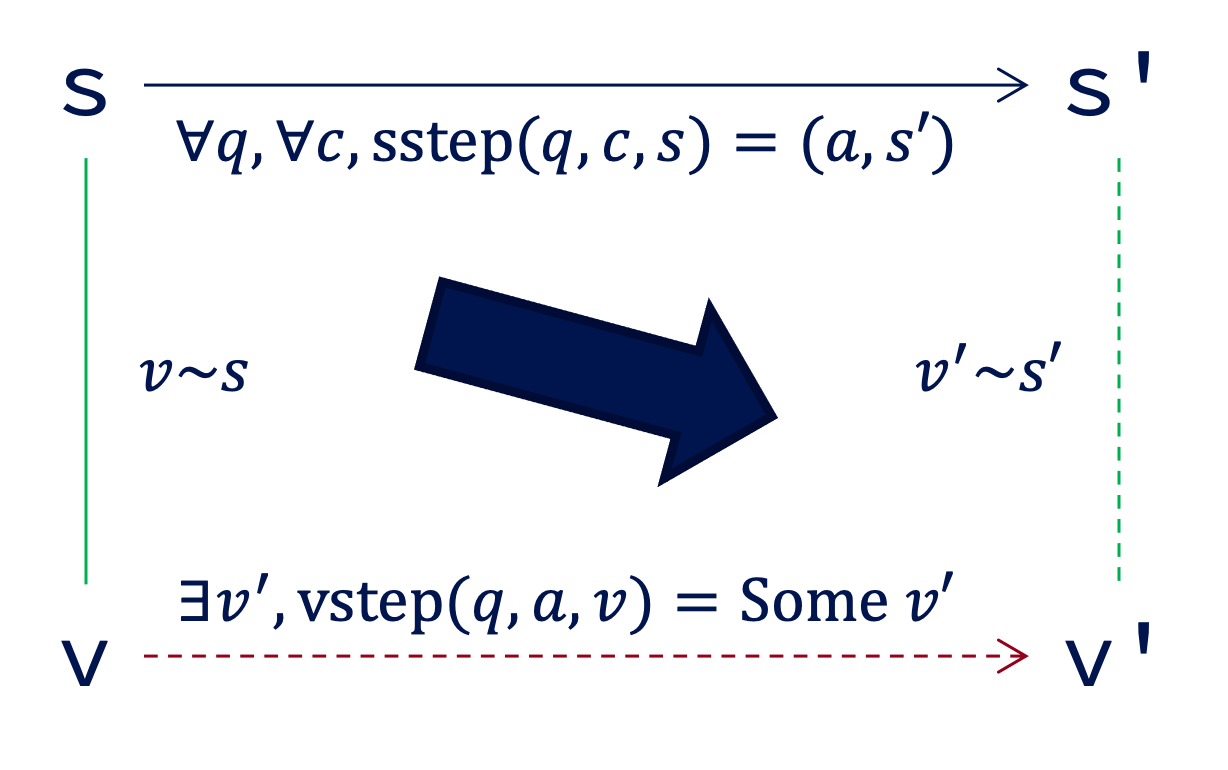
\includegraphics[width=.5\textwidth]{figures/sound}
  \end{center}
\end{itemize}

\subsection{Proving rejection completeness}
The proof of ``any trace consumable by the validator is produceable by
the server'' is by backward induction on the validator's execution
path.  The corresponding server path is constructed based on the
following hypotheses:

\begin{itemize}
\item Any accepting validator step has some server state that reflects the
  post-validation state:
  \begin{align*}
    \tag{RejComplete1}
    \label{eq:rc1}
    \forall(q:Q)(a:A)(v, v':V),\;&\vstep(q,a,v)=\Some{v'}\\
    &\implies\exists s':S,\Reflects{v'}{s'} 
  \end{align*}
\item Any accepting validator step whose post-validation state reflects some
  post-execution server state has a corresponding server step from a
  pre-execution state that reflects the pre-validation state:
  \begin{align*}
    \tag{RejComplete2}
    \label{eq:rc2}
    &\forall(q:Q)(a:A)(v,v':V)(s':S),\\
    &\vstep(q,a,v)=\Some{v'}\wedge\Reflects{v'}{s'}\\
    &\implies\exists(s:S)(c:C),\sstep(q,c,s)=(a,s')\wedge\Reflects{v}{s}
  \end{align*}
  \begin{center}
    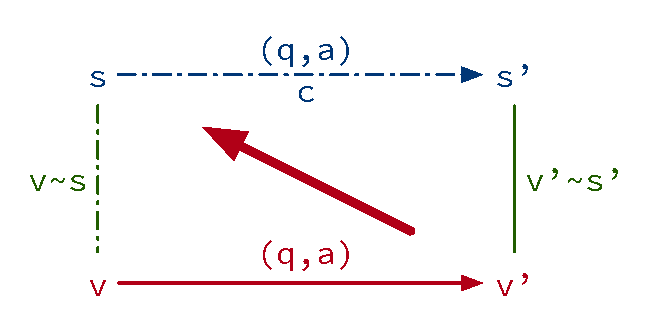
\includegraphics[width=.5\textwidth]{figures/complete}
  \end{center}

\item The initial validator state only reflects the initial server state:
  \begin{equation}
    \tag{RejComplete3}
    \label{eq:rc3}
    \{s\mid\Reflects{v_0}{s}\}=\{s_0\}
  \end{equation}
\end{itemize}

Rejection soundness is proven by forward induction, while rejection completeness
is proven by backward induction.  This is because the choice $c$ is known from
the server step, while unknown from the validator step: Given a validator step,
we cannot predict ``what choices the server will make in the future'', but can
analyze ``what choices the server might have made in the past''.  This proof
method is further explained with the $\Prog$ example:

For specifications written in the $\Prog$ language, the server state is a
mapping from addresses to data; the validation state is a mapping from addresses
to symbolic variables, and constraints over the variables.  A validation state
is accepting if its constraints are satisfiable, {\it i.e.}  there exists an
{\em assignment} of the symbolic variables that can unify the trace with the
server model.  The internal choices made by the server are represented as
symbolic variables.  The assignment maps these variables to the choices' value
at each step, from which we can reconstruct the server's execution path.
\begin{definition}[Bisimulation for $\Prog$ specifications]
  Validator state $v$ {\em simulates} server state $s$ if it contains a
  validation state $(vs,cs)$ that {\em reflects} the server state: (1) There
  exists an assignment $asgn$ that can satisfy the constraints $cs$; and (2) The
  address-variable mapping $vs$ can be {\em instantiated} with the assignment
  (written as ``$vs^{asgn}$'') into an address-data mapping that is equivalent
  with $s$:
  \begin{align*}
    \Reflects v s\quad\triangleq\quad& \exists((vs,cs)\in v)(asgn:\Nat\to\Nat),\satisfy{asgn}
    cs\wedge vs^{asgn}=s\\ vs^{asgn}\quad\triangleq\quad&addr\mapsto
    asgn!(vs!addr)
  \end{align*}
\end{definition}
This bisimulation definition satisfies the hypotheses for proving soundness and
completeness:

Hypotheses~\ref{eq:rs1} and \ref{eq:rc3} are immediate from the initial states'
definition: The initial server state is all-zero map.  The initial validator
state is a singleton that maps all addresses to a variable that is constrained
to have value zero.

\autoref{eq:rc1} is based on the fact that $\vstep_p$ checks the nonemptiness of
the result:
\[\forall q~a~v~v',\vstep_p(q,a,v)=\Some{v'}\implies(\vstep_p'(q,a,v)=v'\wedge\exists (vs,cs)\in v')\]
and that $\vstep_p'$ guards the satisfiability of all constraints in its result:
\[\forall q~a~vs~cs,{(vs,cs)}\in\vstep_p'(q,a,v)\implies\exists asgn,\satisfy{asgn}cs\]

Therefore, any element in the resulting validator state can construct a
simulating server state:
\[\forall asgn~cs~vs~v,(\satisfy{asgn}cs\wedge(vs,cs)\in v)\implies \Reflects{v}{vs^{asgn}}\]

\autoref{eq:rs2} is based on the fact that the pre-validation state must contain
an element that reflects the server's pre-execution state, as defined by the
bisimulation relation.  Given the server's internal choices, we can compute its
execution path.  By induction on the server's execution path, we can construct
the corresponding post-validation state by making the same internal choice and
branch decisions as the server did, and construct the assignment that satisfies
the validator's constraints.

\autoref{eq:rc3} observes that validator design increases the constraints
monotonically.  Therefore, ``assignments that can satisfy the post-validation
constraints'' is a subset of ``assignments that can satisfy the pre-validation
constraints'':
\[\forall q~a~vs~cs~vs'~cs'~asgn,((vs',cs')\in\vstep_p'(q,a,(vs,cs))\wedge\satisfy{asgn} cs')\implies\satisfy{asgn}cs\]

As a result, the corresponding pre-step server state and the internal choice can
be constructed, and proven to perform the server-side step:
\begin{align*}
\forall q~a~vs~cs~vs'~cs'~asgn,\;&(vs',cs')\in\vstep_p'(q,a,(vs,cs))\\
&\implies\sstep_p(q,asgn!(\Fresh{vs}),vs^{asgn})=vs'^{~asgn}
\end{align*}

The intuition here is that the assignment includes ``all choices made by the
server, past and future'', which is narrowed upon more and more observations.
Therefore, the assignment can instantiate all previous validator states into
corresponding servers, and reconstruct the server's execution path by inferring
its internal choices.

